\subsection{前端界面展示}
以下为用户提供的界面截图，用于展示数据导入、研究网格与候选详情。截图中的 29/210、25 个结构、6 个演化子代属于另一界面快照，不与本报告 15 个完成候选的归档合并，也不表示服务器当前正在运行。界面中的曲线与候选状态仅按截图展示，不能替代原始回测数据和独立确认。
\begin{figure}[p]
\centering
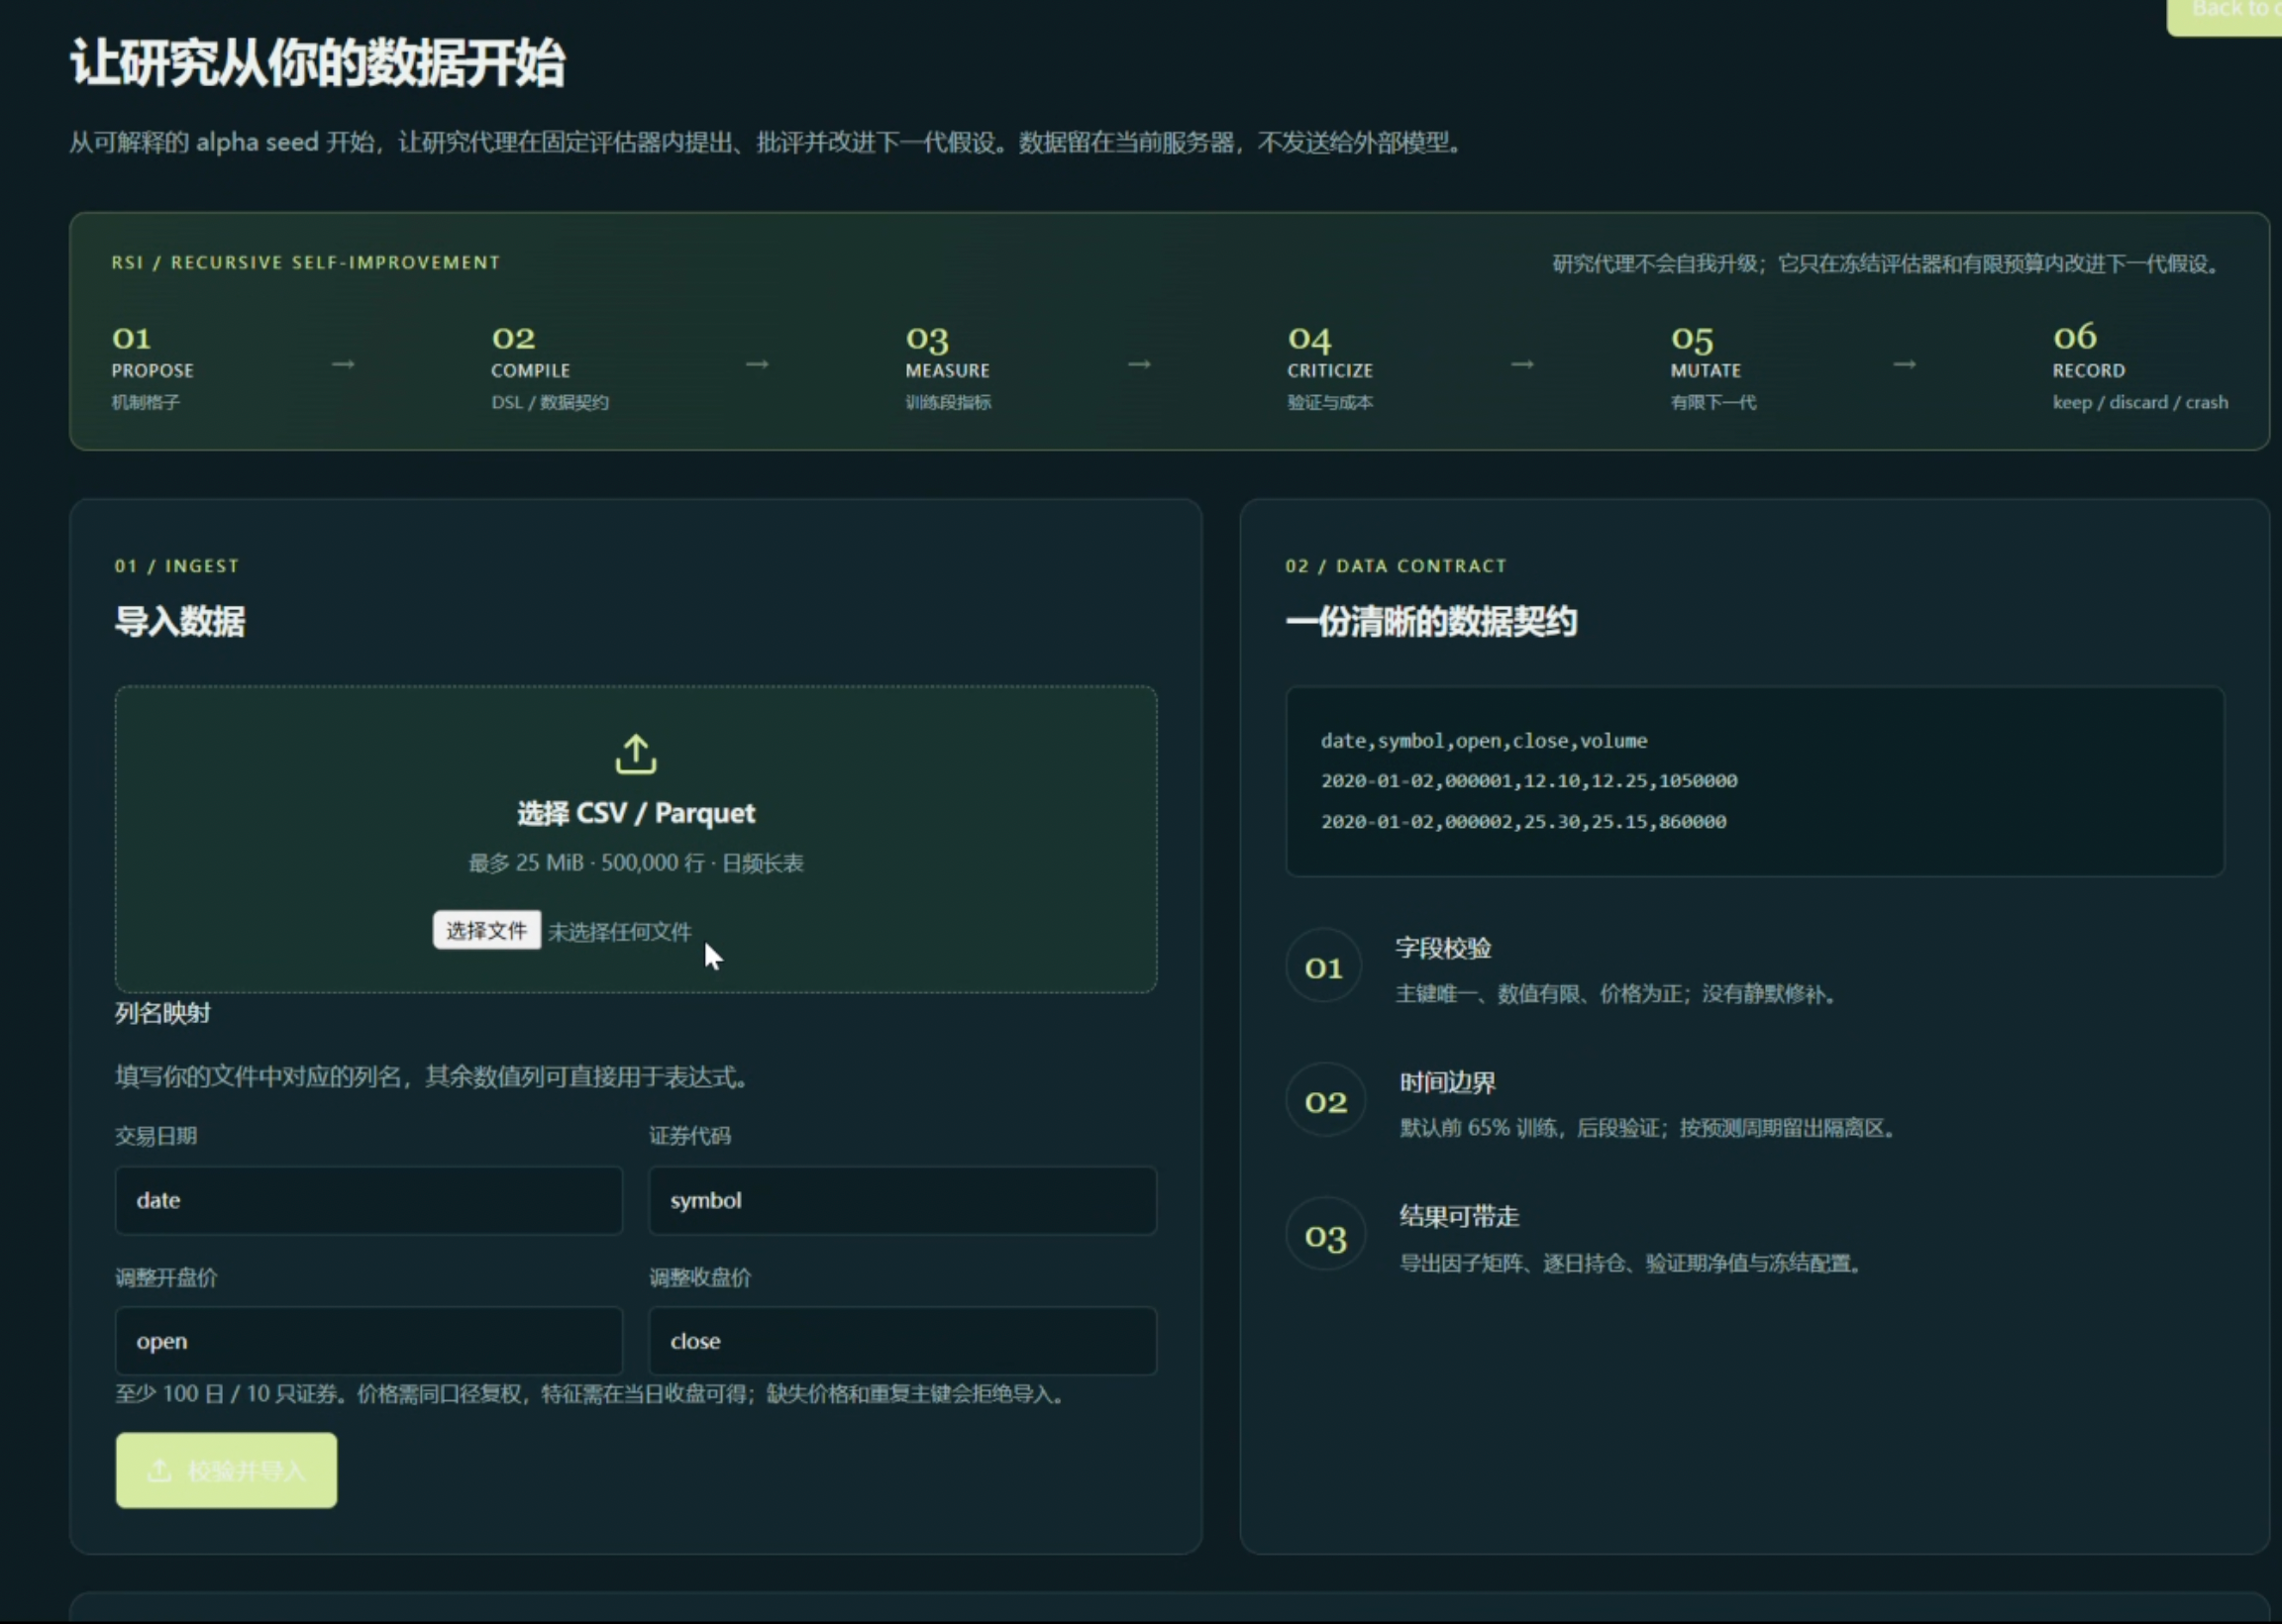
\includegraphics[width=.76\textwidth,height=.7\textheight,keepaspectratio]{figures/frontend/data-intake.png}
\caption{数据导入页：CSV/Parquet 上传、字段映射与数据合同。来源：用户提供的界面截图。}
\end{figure}
\begin{figure}[p]
\centering
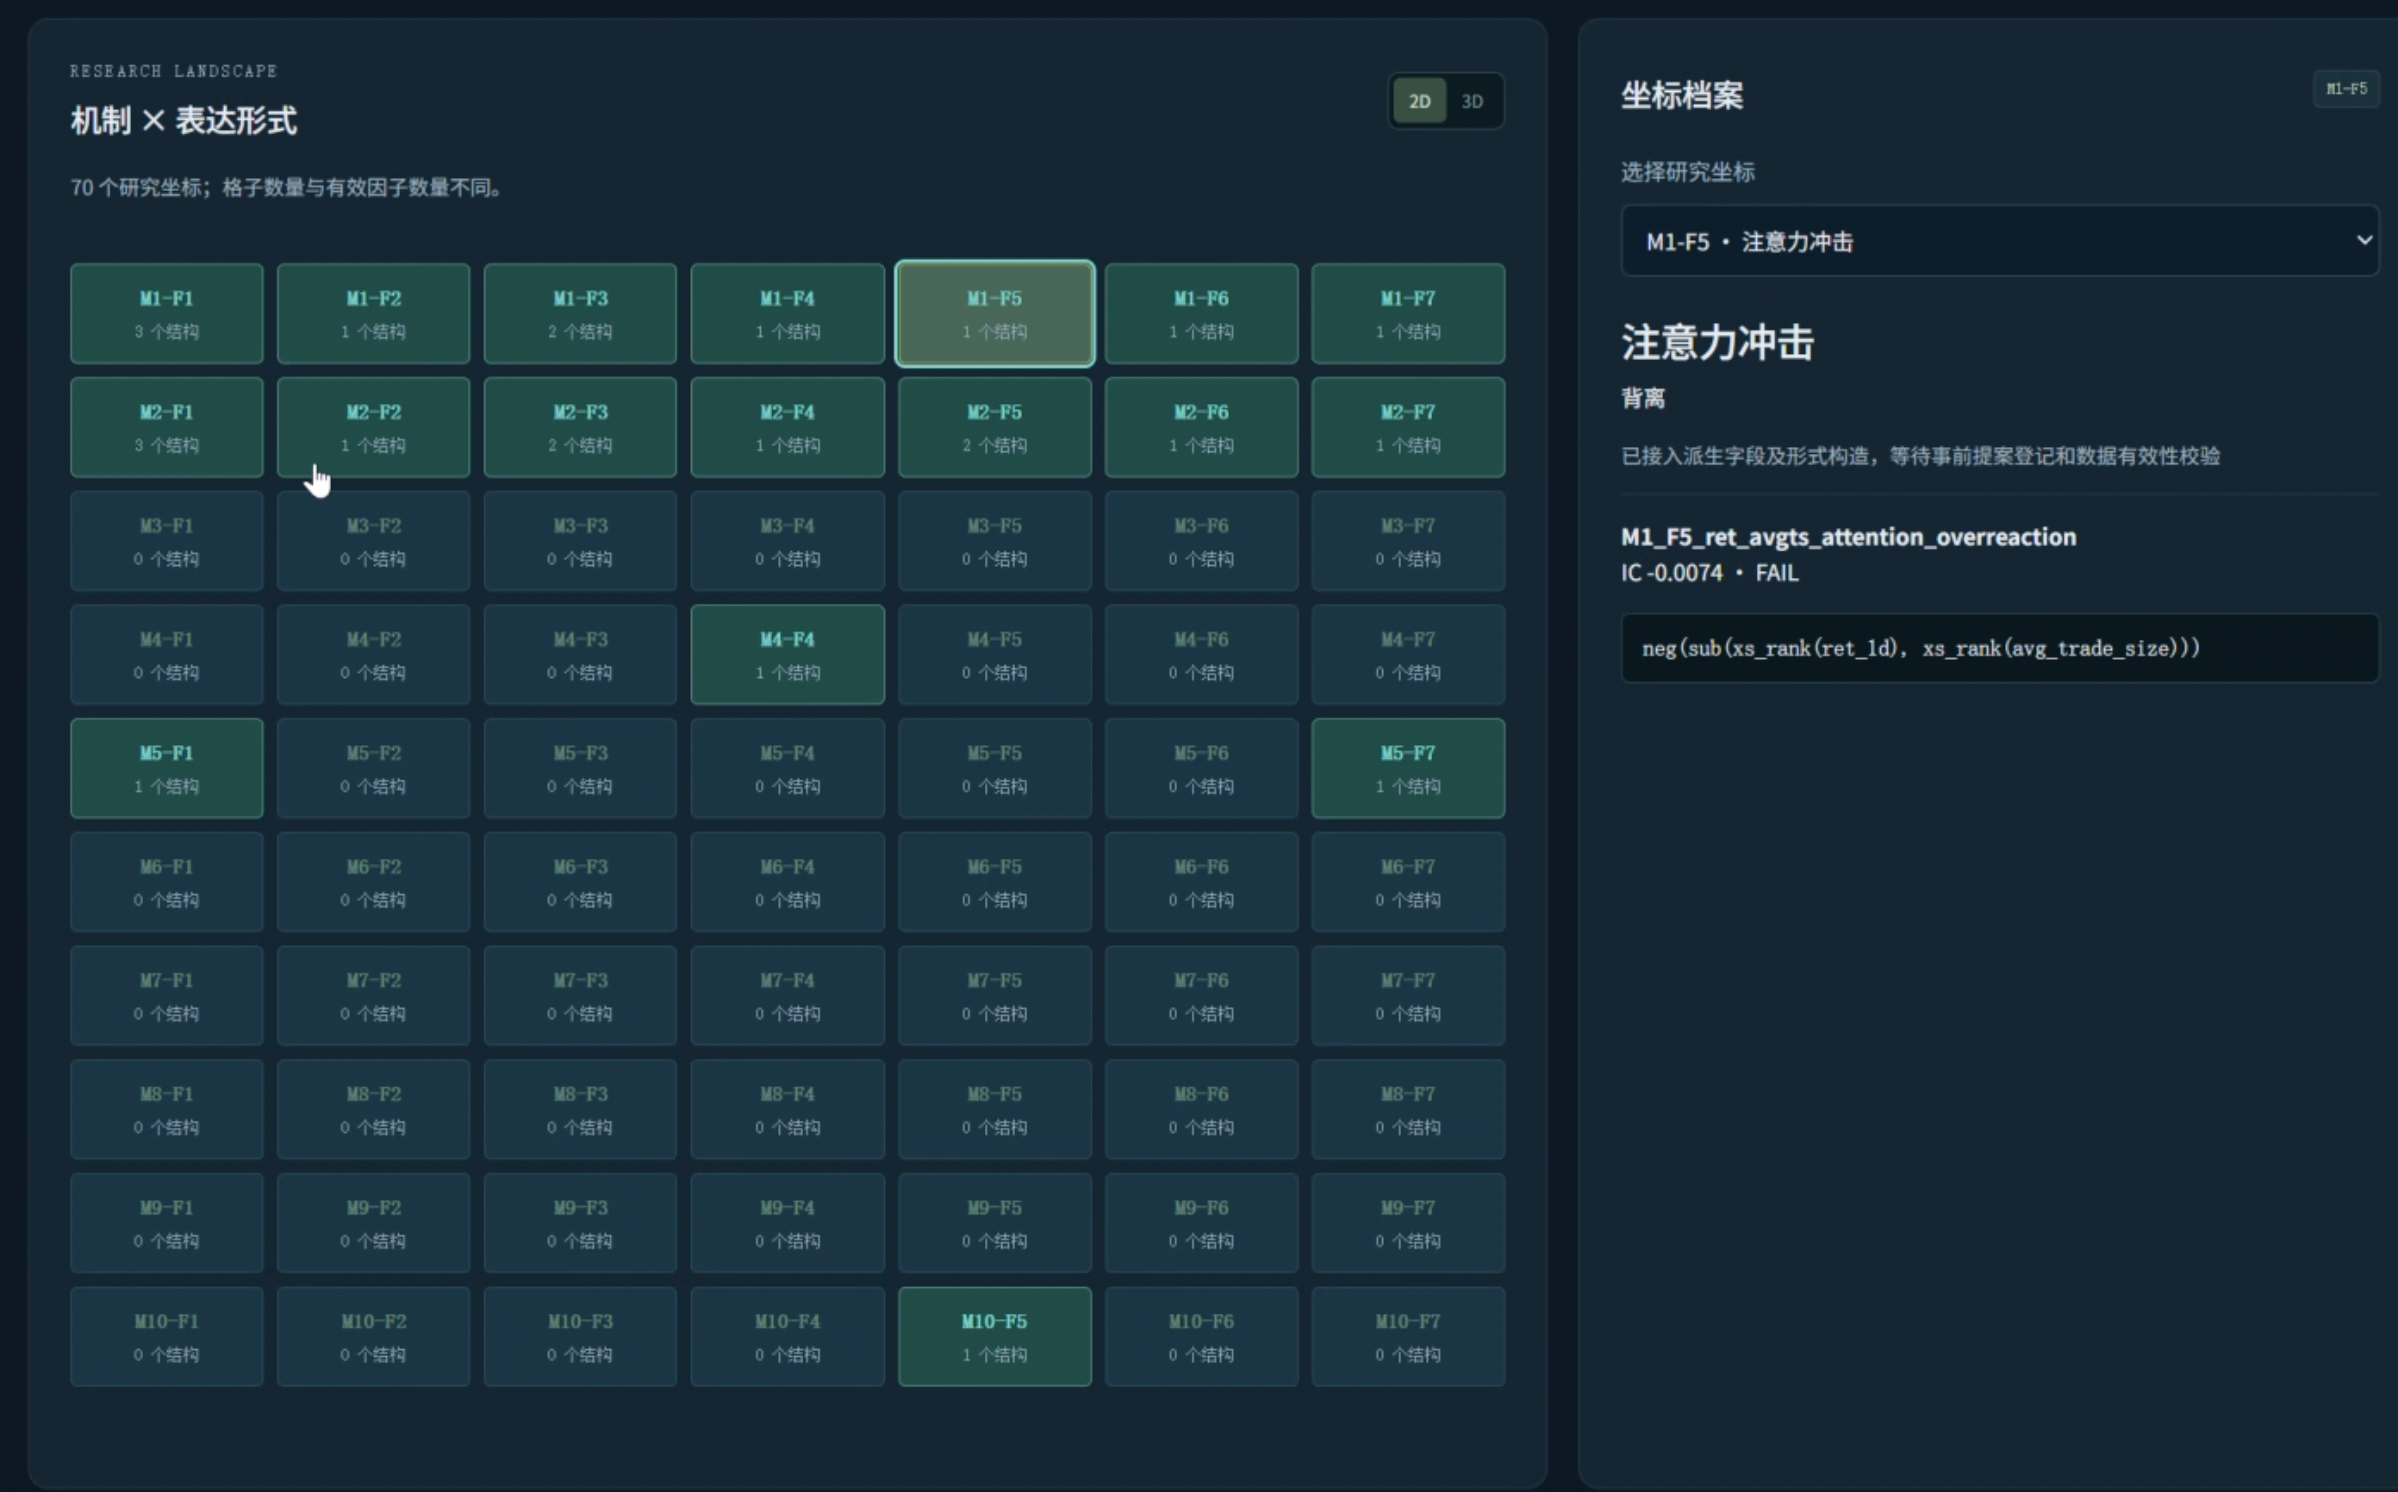
\includegraphics[width=\textwidth,height=.4\textheight,keepaspectratio]{figures/frontend/research-grid.png}
\caption{研究网格：机制与表达形式的组合，以及所选结构的档案。}
\vspace{1em}
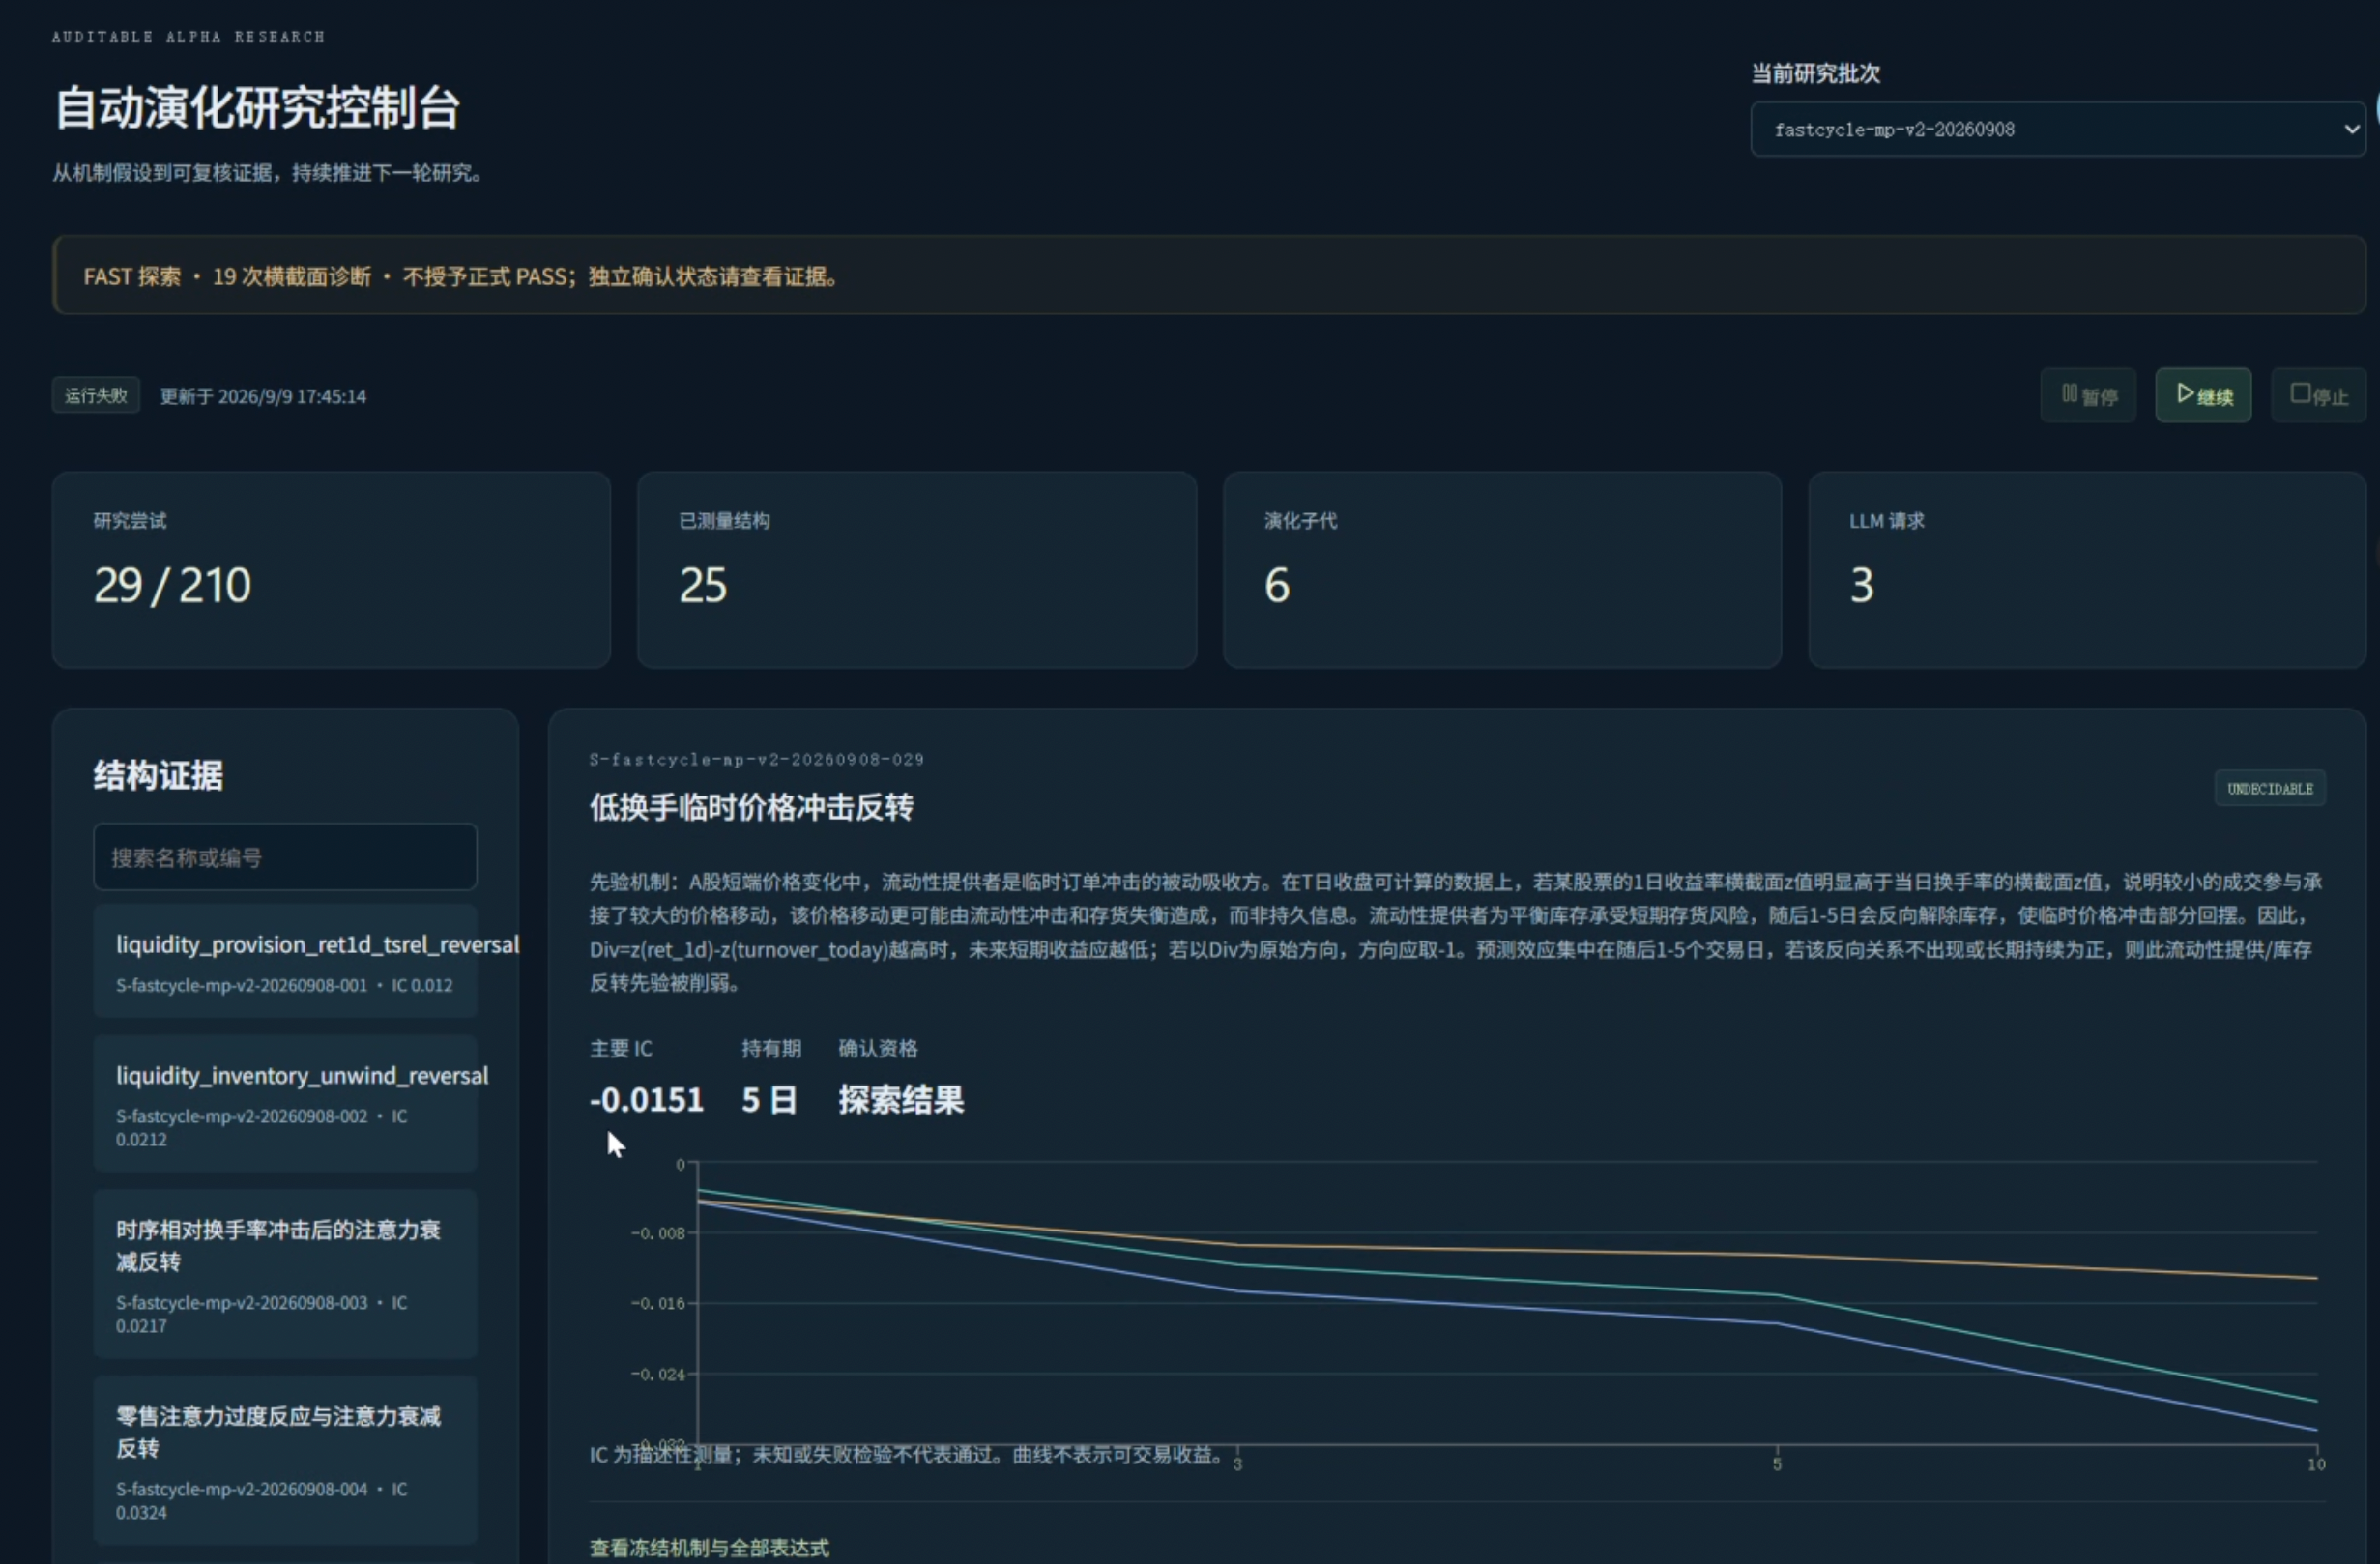
\includegraphics[width=\textwidth,height=.4\textheight,keepaspectratio]{figures/frontend/candidate-detail.png}
\caption{候选详情：显示冻结表达式、研究状态与曲线。截图批次单独保留，不累计为独立确认。}
\end{figure}
\FloatBarrier
